% Chapter 6

\chapter{Development Process \& Tools Used}

\label{ch:development}

%----------------------------------------------------------------------------------------

\section{Coding Guidelines}

\marginpar{The PEPs (Python Enhancement Proposals) are Python's way of
continuously improving the language in a community driven process. Any community
member can submit a proposal for a language change, which is then discussed and
accepted or rejected.}

Coding guidelines are important in order to achieve a consistent style
throughout the codebase. In the Python world, the PEP8 style guide
\cite{pep8:2001} has seen near ubiquitous adaptation and should be used for all
projects in order to aid the legibility of the source code.

\begin{quote}{\slshape
One of Guido's key insights is that code is read much more often than it is
written. The guidelines provided here are intended to improve the readability of
code and make it consistent across the wide spectrum of Python code. As PEP 20
says, ``Readability counts''. \\ \medskip
--- \defcitealias{pep8:2001}{Style Guide for Python Code}\citetalias{pep8:2001} \citep{pep8:2001}
}\end{quote}

\noindent \tangible{} follows most parts of PEP8, with two exceptions:

\begin{itemize}
	\item While line lengths below 80 characters are the ideal case, lines with up
		to 99 characters are still acceptable, if it makes the code more readable.
	\item Errors \texttt{E126--E128}, which specify indentation rules for
		multi-line statements, can be ignored.
\end{itemize}

\noindent The adherence to these coding guidelines are tested automatically by
the test suite. Violations are counted as test failures.

%----------------------------------------------------------------------------------------

\section{Future Imports}\label{sec:development:futures}

While Python 3 has first been released back in 2008, it has still not completely
managed to replace the older 2.x versions. As a result, the \tangible{} codebase
currently targets Python 2.

But in the past year several things have happened that accelerated the adoption
rate of Python 3. Most importantly, several big Linux distributions like Arch
Linux\footnote{\url{https://www.archlinux.org/}} and
Fedora\footnote{\url{http://fedoraproject.org/}} have decided to move to Python
3 as the default Python implementation. Another important factor was the newly
added Python 3 support in big Python frameworks like
Django\footnote{\url{https://www.djangoproject.com/}}.

In view of these facts, the \tangible{} source code is written in a forward
compatible way by adding ``future-imports'' to the top of every code file.
Python provides a module called \texttt{future} which contains backports of
newer language features to older Python versions. By using these imports, the
migration process to newer language versions can be simplified.

In the \tangible{} Project, the following preamble should be added to every
source code file:

\vspace{.5\baselineskip}
\begin{pythoncode}
# -*- coding: utf-8 -*-
from __future__ import print_function, division
from __future__ import absolute_import, unicode_literals
\end{pythoncode}

\noindent This results in the following effects:

\begin{itemize}
	\item The \texttt{\# -*- coding: utf-8 -*-} line tells the Python interpreter
		that this file is UTF8-encoded. In Python 3 UTF8 encoding will become the
		default.
	\item The \texttt{print\_function} import removes the \texttt{print} statement
		and adds a \texttt{print()} function.
	\item When activating the \texttt{division} import, division of two integers
		results in a \texttt{float} value instead of the old, lossy way of returning
		a floored integer. When floor division is explicitly desired, the
		\texttt{//} operator should be used instead.
	\item By importing \texttt{absolute\_import}, Python prioritizes absolute
		imports over relative imports. This fixes a few issues with import name
		clashes.
	\item The \texttt{unicode\_literals} import is the one with the most
		consequences of all the future imports listed above. It changes the default
		type of strings from bytestrings to unicode objects. By eliminating this
		Python 2/3 consistency from the beginning, many hard to spot migration bugs
		can be prevented.
\end{itemize}

\noindent The choice of future imports is based on the article \emph{Quick Tips
on Making Your Code Python 3 Ready} by Hristo Deshev \cite{deshev:2012}

%----------------------------------------------------------------------------------------

\section{Testing}

\begin{quote}{\slshape
More than the act of testing, the act of designing tests is one of the best bug
preventers known. The thinking that must be done to create a useful test can
discover and eliminate bugs before they are coded — indeed, test-design thinking
can discover and eliminate bugs at every stage in the creation of software, from
conception to specification, to design, coding and the rest.\\ \medskip
--- \defcitealias{beizer:2003}{Boris Beizer}\citetalias{beizer:2003} \citep{beizer:2003}
}\end{quote}

\noindent Testing is not a question of "whether", but rather a question of
"how". By having a high test coverage of your code base, code can be changed
without any fear of overlooking newly introduced bugs. The TDD\footnote{Test
Driven Development} methodology greatly aids both the process of writing tests,
as well as the process of writing software. By writing tests before actually
implementing the code leads to better structured, more easily testable code with
less bugs than if testing features after their implementation.

This section can be divided into three subsections: Writing the tests, running
the tests and measuring test coverage.

\subsection{Writing Tests}

\tangible{} uses the pytest\footnote{\url{http://pytest.org/}} framework for
writing tests. pytest provides both tools for easier and more lightweight
testing as well as an easy way for test discovery.

In contrast to Python's builtin \texttt{unittest} module, which was heavily
inspired by Java, pytest does not require the developer to use explicit methods
for expressing assertions like \texttt{assertEquals} or \texttt{assertGreater}.
Instead it relies on the \texttt{assert} keyword while still providing useful
error messages by using language reflection.

A simple test could just look like the following example:

\vspace{.5\baselineskip}
\begin{pythoncode}
def test_the_answer():
    assert 19 + 23 == 42
\end{pythoncode}

\noindent In contrast, the \texttt{unittest} version would look like this:

\vspace{.5\baselineskip}
\begin{pythoncode}
import unittest
class TestTheAnswer(unittest.TestCase):
    def testIt(self):
        self.assertEquals(19 + 23, 42)
\end{pythoncode}

As the Zen of Python \cite{pep20:2004} states, \emph{``Simple is better than
complex.''}. Therefore the Pytest version should be preferred over using
\texttt{unittest}.

But simpler asserts are not the only advantage that pytest offers over unittest.
Another feature that has been used extensively in \tangible{} is parametrized
testing. By specifying a set of possible values for the test parameters using
the \texttt{pytest.mark.parametrize} decorator, multiple tests are generated
from a single test function. If one of five input values makes the test fail,
the test result would be 4 successful tests out of a total of 5, whereas putting
all the values to be checked in a nonparametrized function would lead to a
single failing test.

Here is an example of a parametrized test from the \tangible{} test suite:

\vspace{.5\baselineskip}
\begin{pythoncode}
import pytest
from tangible import scales

@pytest.mark.parametrize(('param', 'clamp', 'expected'), [
    (2, False, 10),
    (3.5, False, 17.5),
    (6, False, 30),
    (6, True, 20),
])
def test_linear(param, clamp, expected):
    domain, codomain = (2, 4), (10, 20)
    scale = scales.linear(domain, codomain, clamp)
    assert scale(param) == expected
\end{pythoncode}


\subsection{Running Tests}

pytest offers highly customizable test discovery out of the box. After
configuring the patterns to be used for detecting tests, the suite can be run
by simply issueing \texttt{py.test} in the main project directory.

But manually running tests is a step that's often forgotten while developing.
Tests are better when they're fully automated. Travis CI
(\url{https://travis-ci.org/}) is a startup company that offers free continuous
integration for open source projects. A minimal configuration file is all that's
needed to get everything up and running. The test results are presented in an
easy to understand manner in the web browser:

\begin{figure}[H]
	\centering
	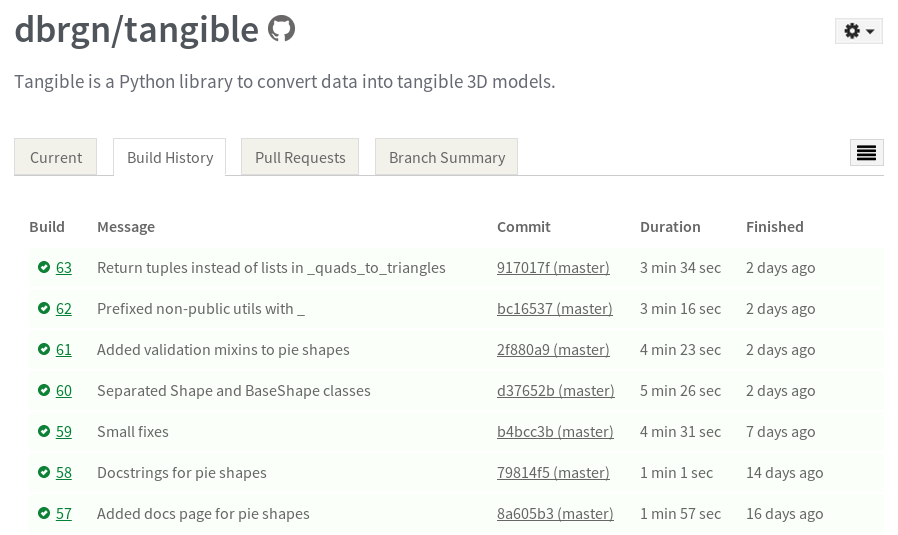
\includegraphics[width=\textwidth]{images/travis.png}
	\caption{Travis CI}
	\label{img:travis}
\end{figure}

\subsection{Measuring Test Coverage}

Simply having many tests does not necessarily mean that the code is well tested.
A high test coverage coes not either, but it's a good indicator on how many
lines of code have been hit by the tests, and how many haven't.

In the \tangible{} project coverage is measured through the
coverage.py\footnote{\url{http://nedbatchelder.com/code/coverage/}} module. The
result is displayed each time the test suite runs thanks to the
pytest-cov\footnote{\url{https://pypi.python.org/pypi/pytest-cov}} plugin for
pytest.

Change in test coverage is tracked by the Coveralls.io
(\url{https://coveralls.io/}) service. The current coverage can be included in
the README file by embedding a dynamic image from the Coveralls server. This
way, the current coverage is always visible.

%----------------------------------------------------------------------------------------

\section{Tools Used}

During the time of this thesis, the following tools have been used:

\begin{itemize}
	\item The Vim text editor for editing both program source code and
		documentation.\\ \url{http://www.vim.org/}
	\item Flake8 for coding style checks and static code analysis.\\
		\url{https://flake8.readthedocs.org/}
	\item pytest for running the test suite.\\
		\url{http://pytest.org/}
	\item Travis CI for automated testing.\\
		\url{https://travis-ci.org/}
	\item Coveralls for automated test coverage measuring.\\
		\url{https://coveralls.io/}
	\item OpenSCAD to convert the generated model code to actual STL files.\\
		\url{http://www.openscad.org/}
	\item Makerbot / Makerware to test-print a few of the generated 3D models.\\
		\url{http://www.makerbot.com/makerware/}
	\item \LaTeX{} for typesetting this project documentation.\\
		\url{http://www.latex-project.org/}
	\item Sphinx for generating the online user documentation.\\
		\url{http://sphinx-doc.org/}
	\item Git and Github for version control.\\
		\url{http://git-scm.com/} \url{https://github.com/}
\end{itemize}
